\documentclass[12pt]{article}
\usepackage[utf8]{inputenc}
%\usepackage{csquotes}
\usepackage{graphicx}
\graphicspath{ {pictures/} }
\usepackage{caption}
\usepackage{subcaption}
\usepackage[a4paper,width=150mm,top=25mm,bottom=25mm,bindingoffset=6mm]{geometry}
\usepackage[english, ngerman]{babel}
\usepackage{amsthm,etoolbox, amsmath, amssymb}
\usepackage{enumitem}   
\usepackage[nottoc]{tocbibind}
\usepackage{hyperref}
\usepackage{wrapfig}
\usepackage{color} 
\usepackage{algorithm}
\usepackage{algpseudocodex}
\usepackage{aligned-overset}
\usepackage [autostyle, german = quotes]{csquotes}
\usepackage{tikz}
\usepackage{pgffor}
\usepackage{listings}
\usepackage{fancyhdr}
\MakeOuterQuote{"}

\AddToHook{cmd/section/before}{\clearpage}

\theoremstyle{plain}
\newtheorem{thm}{Theorem}
\newtheorem{lem}[thm]{Lemma}
\newtheorem{prop}[thm]{Proposition}
\newtheorem{cor}[thm]{Korollar}

\theoremstyle{definition}
\newtheorem{definition}[thm]{Definition}
\newtheorem{ex}[thm]{Beispiel}

\theoremstyle{remark}
\newtheorem{rem}[thm]{Bemerkung}

\makeatletter
\@addtoreset{thm}{section}% Reset theorem counter with every section
\@addtoreset{thm}{subsection}
\@addtoreset{thm}{subsubsection}
\newcommand{\theoremprefix}{}
\let\thetheoremsaved\thethm
\renewcommand{\thethm}{\theoremprefix\thetheoremsaved}
\let\sectionsaved\section
\patchcmd{\@startsection}{\par}{\renewcommand{\theoremprefix}{\csname the#1\endcsname.}}{}{}
\makeatother

\setlength{\jot}{10pt}
\setlength{\headheight}{15pt}

\newcommand*\circled[1]{\tikz[baseline=(char.base)]{%
            \node[shape=circle,fill=blue!20,draw,inner sep=2pt] (char) {#1};}}

\usepackage[style=alphabetic, firstinits=true, backend=biber, sorting=nyt, doi=false, isbn=false, url=true, maxbibnames=99]{biblatex}
\DeclareNameAlias{default}{family-given}
\addbibresource{references.bib}

\title{Thesis Title}
\author{Author Name}
\date{Day Month Year}

\setlength\parindent{0pt}

\begin{document}
	\begin{titlepage}
	\begin{center}
		\vspace*{1cm}
		
\includegraphics{TU_Logo_kurz_1c_schwarz.eps}\\
		\Large
		Technische Universität Berlin\\
		Institut für Mathematik
		\vspace*{1cm}



		\Huge
		\textbf{Numerischer Wertebereich}
		
		\vspace{0.5cm}
		\LARGE
		und Anwendung auf das Lax-Wendroff-Verfahren
		
		\vspace{1.5cm}
		
		\textbf{Sijun John Tu}
		
		\vfill
		
		Bachelorarbeit \\
		zur Erlangung des Grades\\
		Bachelor of Science \\
		im Fach Mathematik
		
		\vspace{0.8cm}

		
		
		Betreuerin: Frau Dr. Agnes Radl\\
		Zweitgutachterin: Prof. Dr. Tanja Eisner \\
		
	\end{center}
\end{titlepage}
	
\subsubsection*{Abstract}

    In this paper, we investigate the so-called numerical value range of a linear, bounded operator in a Hilbert space. Similar to the spectrum of an operator, the numerical range of values helps to determine certain properties of the corresponding operator to be investigated. In doing so, we will often encounter relations between there two invariants. The main objective of this section is the so-called Power Inequality, a statement about the numerical radius of powers of an operator, as well as the norm property of the numerical radius. In particular, an algorithm is presented and implemented, which numerically approximates the numerical value for a finite-dimensional operator. In the final chapter of the thesis, an application of the numerical value range in numerical mathematics is considered.


	\thispagestyle{empty}
\section*{Eidesstattliche Erklärung}

Hiermit erkläre ich, dass ich die vorliegende Arbeit selbstständig und eigenhändig sowie ohne unerlaubte fremde Hilfe und ausschließlich unter Verwendung der aufgeführten Quellen und Hilfsmittel angefertigt habe.\\

Die selbstständige und eigenhändige Anfertigung versichert an Eides statt:\\\\\\\\\\
Berlin, den \today \\[5cm]
\rule{10cm}{0.4pt}\\
Sijun John Tu
	\tableofcontents
	\thispagestyle{empty}
	% \addtocontents{toc}{\protect\thispagestyle{empty}}
	\setcounter{page}{0}

	
\section*{Notation}
Mathematical conventions and notation used in this thesis:

\begin{center}
    \renewcommand{\arraystretch}{1.5}
    \begin{tabular}{ c l }
        
        $\mathbb{R}$ & the real numbers \\
        $\sqcup$ & disjoint set union \\
        $\mathcal{N}(\mu, \sigma^2)$ & Gaussian distribution with mean $\mu$ and variance $\sigma^2$
    \end{tabular}
\end{center}

Additionally, we introduce the following conventions to describe various elements from different mathematical objects to make the notations and their meaning as consistent as possible:

\begin{center}
    \renewcommand{\arraystretch}{1.5}
    \begin{tabular}{c l}
        $\mathcal{S}$ & set of heartbeat samples \\
        $s_i \in \mathbb{R}^L$ & seqeunce of ECG measurements \\
        $\mathcal{K}^X$ & arrhythmia detection model trained on some training data $X$


    \end{tabular}
\end{center}

	\addcontentsline{toc}{section}{Notation}

	\listoffigures

	\pagestyle{fancy}
	\fancyhf{}
	\fancyhead[L]{\leftmark}
	\fancyfoot[R]{\thepage}


	\section{Mathematische Grundlagen}
	Der numerische Wertebereich und Radius werden in einem Hilbertraum-Setting für lineare und beschränkte Operatoren definiert. Daher werden in diesem Abschnitt die grundlegenden Ergebnisse und Definitionen aus der Theorie der Hilberträumen in kompakter Weise erläutert, aber ohne Beweis aufgeführt. Details können den Standardwerken zur Funktionalanalysis entnommen werden, siehe \parencite[][Kapitel 5, 6]{werner2006funktionalanalysis} oder auch \parencite[][Kapitel 1,2, 6, 7]{conway2019course}.

\subsection{Hilberträume}

Sei $\mathbb{K}$ ein Körper. Im Kontext dieser Arbeit wird $\mathbb{K}$ meistens der Körper der komplexen Zahlen $\mathbb{C}$ sein, seltener auch der Körper der reellen Zahlen $\mathbb{R}$. Üblicherwei\-se wird die Notation $\mathbb{K} \in \{\mathbb{C}, \mathbb{R}\}$ eingeführt. Auf einem Vektorraum $X$ über $\mathbb{K}$ definieren wir das Skalarprodukt als eine Abbildung, die zwei Elemente aus dem Vektorraum auf ein Element des zugrundeliegenden Körpers wie folgt abbildet:

\begin{definition}[Skalarprodukt]
    Sei X ein Vektorraum über $\mathbb{K}$. Dann ist ein Skalarprodukt auf X eine Abbildung
    \begin{align*}
        \left<\cdot ,\cdot \right> : X \times X \longrightarrow \mathbb{K} \; ,
    \end{align*}
    welche folgende Eigenschaften für alle $ x,y,z \in X$ und $a, b \in \mathbb{K}$ erfüllt: \begin{enumerate}[label=(\roman*)]
        \item Linearität im ersten Argument: \begin{align*}
            \left< a x + b y, z \right> = a \left< x , z \right> +b \left< y, z \right>
        \end{align*}
        \item konjugierte Symmetrie: \begin{align*}
            \left< x,y \right> = \overline{\left< y,x \right>}
        \end{align*}
        \item  positive Definitheit: \begin{align*}
            \left< x,x \right> \ge 0 \\
            \left< x,x \right> = 0 \iff x = 0
        \end{align*}
    \end{enumerate}
\end{definition}

Einen Vektorraum ausgestattet mit einem Skalarprodukt nennt man auch einen Prä\-hilbert\-raum. Ein Hilbertraum ist dann ein voll\-ständiger Prä\-hilbert\-raum, wobei als Norm die vom Skalarprodukt induzierte Norm betrachtet wird (man mache sich bewusst, dass es sich dabei wirklich um eine Norm handelt!).

\begin{definition}[Hilbertraum]
    Sei $X$ ein Prähilbertraum mit Skalarprodukt $\left<\cdot, \cdot \right>$ und induzierter Norm $\| \cdot \| = \sqrt{\left<\cdot, \cdot \right>}$. Dann ist $X$ ein Hilbertraum, falls $X$ vollständig bezüglich $\| \cdot \|$ ist.
\end{definition}

\begin{ex} \label{ex:standard_skp}
    Das Standardskalarprodukt auf $\mathcal{H}=\mathbb{C}^n$ ist wie folgt definiert: Für Vektoren \begin{align*}
        x = \begin{pmatrix}
            x_1 \\ \vdots \\ x_n
        \end{pmatrix} \; , \;
        y = \begin{pmatrix}
            y_1 \\ \vdots \\ y_n
        \end{pmatrix}
    \end{align*}
    aus $\mathcal{H}$
    ist \begin{align*}
        \left<x,y \right> = \sum_{k=1}^n {x_k \overline{y_k}} \;\; .
    \end{align*} 
    $\mathbb{C}^n$ mit dem so definierten Skalarprodukt ist ein Hilbertraum.
\end{ex}

Nun können lineare, beschränkte Operatoren auf einem Hilbertraum definiert werden.

\begin{definition}[linearer, beschränkter Operator]
    Sei $T: \mathcal{H} \longrightarrow \mathcal{H}$ eine Abbildung auf einem Hilbertraum $\mathcal{H}$. Dann ist $T$ \begin{enumerate}[label=(\roman*)]
        \item linear, falls für alle $x,y \in \mathcal{H}$ und $a ,b \in \mathbb{K}$ gilt: \begin{align*}
            T(a x + b y) = a Tx + b Ty
        \end{align*}
        \item beschränkt, falls ein $M > 0 $ existiert, sodass für alle $x \in \mathcal{H}$ gilt: \begin{align*}
            \| Tx \| \le Mx
        \end{align*}
    \end{enumerate}
    Der Raum aller linearen, beschränkten Operatoren auf $\mathcal{H}$ wird mit $\mathcal{L}(\mathcal{H})$ bezeichnet. Ausgestattet mit der Operatornorm $\|T\| = \sup_{\|x\|=1} \|Tx\| $ ist $\mathcal{L}(\mathcal{H})$ sogar ein Banachraum, solange $\mathcal{H}$ ein Hilbertraum ist. 
\end{definition}

Falls $\mathcal{H}$ endlichdimensional ist, kann jeder lineare, beschränkte Operator mit einer Matrix identifiziert werden. Das Konzept der adjungierten Matrix kann auch für unendlichdimensionale Hilberträume verallgemeinert werden und führt auf den Begriff des adjungierten Operators.

\begin{definition}[adjungierter Operator]
    Für $T\in \mathcal{L}(\mathcal{H})$ heißt der eindeutige Operator $T^*\in \mathcal{L}(\mathcal{H})$ mit $\left< Tx,y \right> = \left< x,T^*y \right>$ für alle $x, y \in \mathcal{H}$ der zu $T$ adjungierte Operator.  
\end{definition}

Es ist nützlich, bestimmte Klassen von Operatoren in Hilberträumen näher zu betrachten, daher werden nun unitäre, normale und selbst-adjungierte Operatoren definiert.

\begin{definition}[selbst-adjungierte, normale, unitäre Operatoren]
    Ein linear, beschränkter Operator $T \in \mathcal{L}(\mathcal{H})$ heißt
    \begin{itemize}
        \item selbst-adjungiert, falls $T=T^*$
        \item normal, falls $T$ und $T^*$ kommutieren, das heißt $TT^*=T^*T$
        \item unitär, falls $T$ invertierbar und $T^{-1}=T^*$
    \end{itemize}
\end{definition}

Manchmal ist es auch hilfreich, Projektionen von einem Hilbertraum auf einen Unterraum $V$ zu betrachten. Insbesondere werden wir die sogenannte orthogonale Projektion benötigen, um ein Theorem über die Konvexitätseigenschaft des numerischen Wertebereichs zu beweisen. Die orthogonale Projektion bildet ein beliebiges Element $x$ aus dem Hilbertraum auf das eindeutige Element im Unterraum $V$ ab, sodass der Abstand zwischen diesen beiden Elementen genau dem Abstand zwischen $x$ und $V$ entspricht. 

\begin{thm}[Orthogonale Projektion] \label{thm_orth_proj}
    Sei $\mathcal{H}$ ein Hilbertraum und $V \subseteq \mathcal{H}$ ein abgeschlossener, nicht-leerer, linearer Unterraum. Dann existiert zu jedem $x \in \mathcal{H}$ ein eindeutiges Element $Px \in V$, sodass $\|x-Px\|=d(x, V)= \inf_{v\in V} \|x-v\|$. Die Abbildung \begin{align*}
        P: \mathcal{H} \longrightarrow \mathcal{H} \; \; , \; x \mapsto Px
    \end{align*}
    heißt die orthogonale Projektion von $\mathcal{H}$ auf $V$. Außerdem ist $P \in \mathcal{L}(\mathcal{H})$ und selbst-adjungiert. 
\end{thm}

\subsection{Spektraltheorie}

Das Konzept von Eigenwerten und -vektoren aus der linearen Algebra kann auch auf unendlichdimensionale Vektorräume verallgemeinert werden. Dafür werden folgende Mengen definiert:

\begin{definition}
    Sei $\mathcal{H}$ ein komplexer Hilbertraum und $T\in \mathcal{L}(\mathcal{H})$. Dann definiert man: \begin{itemize}
        \item die Resolventenmenge von $T$ \begin{align*}
            \rho(T) := \left\{ \lambda \in \mathbb{C}: \lambda -T \text{ ist bijektiv} \right\}
        \end{align*}
        \item das Spektrum von $T$
        \begin{align*}
            \sigma(T)=\mathbb{C} \setminus \rho(T)
        \end{align*}
        
        \item das Punktspektrum von $T$ 
        \begin{align*}
            \sigma_{p}(T) := \left\{ \lambda \in \mathbb{C}: \lambda -T \text{ ist nicht injektiv} \right\}
        \end{align*}
        \item das approximative Punktspektrum von $T$ 
        \begin{align*}
            \sigma_{app}(T)=\{ \lambda \in \mathbb{C}: \exists \{x_n\}_n \in \mathcal{H} \text{ sd. } \|x_n\|=1  \text{ für alle $n\in\mathbb{N}$ und } \\ 
            \|(T-\lambda)x_n \| \rightarrow 0 \text{ für } n \rightarrow \infty \}
        \end{align*}
        \item den Spektralradius von $T$ \begin{align*}
            r(T)=\sup_{\lambda \in \sigma(T)} |\lambda|
        \end{align*}
    \end{itemize}
\end{definition}

Dabei gilt folgende wichtige Inklusion \parencite[][Problem 78]{halmos2012hilbert}.

\begin{lem} \label{lem:point_approx_spec}
    Der Rand vom Spektrum ist enthalten im approximativen Punktspektrum, das heißt $\partial \sigma(T) \subseteq \sigma_{app}(T)$
\end{lem}


\subsection{Schurzerlegung}

Es ist bekannt, dass das Spektrum eines Operators invariant unter Ähnlich\-keits\-trans\-for\-ma\-tionen ist. Eine schwächere Aussage gilt auch für den numerischen Wertebereich - nämlich nur noch für unitäre Ähnlichkeitstransformationen. Diese Eigenschaft werden wir später in Proposition \ref{prop:properties_numran} zeigen. Daher ist es im Endlichdimensionalen sinnvoll, die sogenannte Schur-Zerlegung von Matrizen zu betrachten; diese erlaubt es, jede Matrix als eine unitär ähnliche obere Dreiecksmatrix darzustellen. Sie wurde 1909 von Issai Schur entdeckt und bewiesen in \parencite{schur1909charakteristischen}.

\begin{thm}[Schur-Zerlegung]
    Sei $A \in Mat_{n,n}(\mathbb{C})$. Dann existiert eine unitäre Matrix $U\in Mat_{n,n}(\mathbb{C})$ sodass 
    \begin{align*}
        U^*AU = R
    \end{align*}
    wobei $R$ eine obere Dreiecksmatrix ist.
\end{thm}

Findet man also so eine Zerlegung einer Matrix, dann lassen sich die Eigenwerte direkt von der Diagonalen von $R$ ablesen.


	
	\section[Numerischer Wertebereich und numerischer Radius]{Numerischer Wertebereich und \\numerischer Radius}
	\section{Project introduction}

\begin{frame}
    \frametitle{Machine Learning Pipeline}
    \tikz{
            \node[circle,fill=Button1,inner sep=3pt] (c) at (0,0){};
            \node[circle,fill=Button2,inner sep=3pt] (c) at (0.5,0){};
            \node[circle,fill=Button3,inner sep=3pt] (c) at (1,0){};
        }~~~~~~\textcolor{gold}{Figure: }High-level machine learning pipeline
    \begin{figure}[h]
        
        \centering
        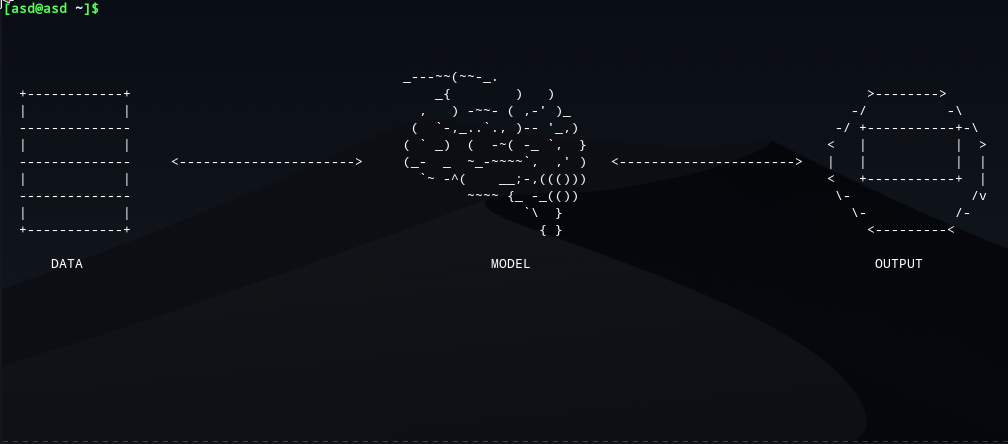
\includegraphics[scale=0.45]{ml_pipeline.png}
    \end{figure}
\end{frame}



\begin{frame}{Anomaly detection using privacy-preserving, synthetic time series data}
    
    \begin{itemize}
        \item Problem
        \begin{itemize}
            \item ML models are very \alert{data hungry}.
            \item In many cases sharing data comes with \alert{privacy risks}.
        \end{itemize}
        \item Solution:
        \begin{itemize}
            \item Promising solution: \alert{synthetic data} with privacy guarantees!
            \item Synthetic data with \alert{differential private} (DP) guarantees is a promising solution to ensure privacy independent of downstream task.
        \end{itemize}
        \item BUT:
        \begin{itemize}
            \item \alert{Privacy-Utility-Tradeoff}: Commonly, a gain in privacy results in a loss of utility. 
            \item For \alert{anomaly detection} this might not be the case (?).
        \end{itemize}
    \end{itemize}
    Goal: generate useful and privacy-preserving ECG data for anomaly detection (heartbeat arrhythmia).
\end{frame}


\begin{frame}{Structure}
    
    \begin{figure}[h]
        \begin{flushleft}
            \tikz{
            \node[circle,inner sep=3pt] (c) at (-0.5,0){};
            \node[circle,fill=Button1,inner sep=3pt] (c) at (1.0,0){};
            \node[circle,fill=Button2,inner sep=3pt] (c) at (1.5,0){};
            \node[circle,fill=Button3,inner sep=3pt] (c) at (2.0,0){};
        }~~~~~~\textcolor{gold}{Figure: }Structure of Experiment pipeline
        \end{flushleft}
        \centering
        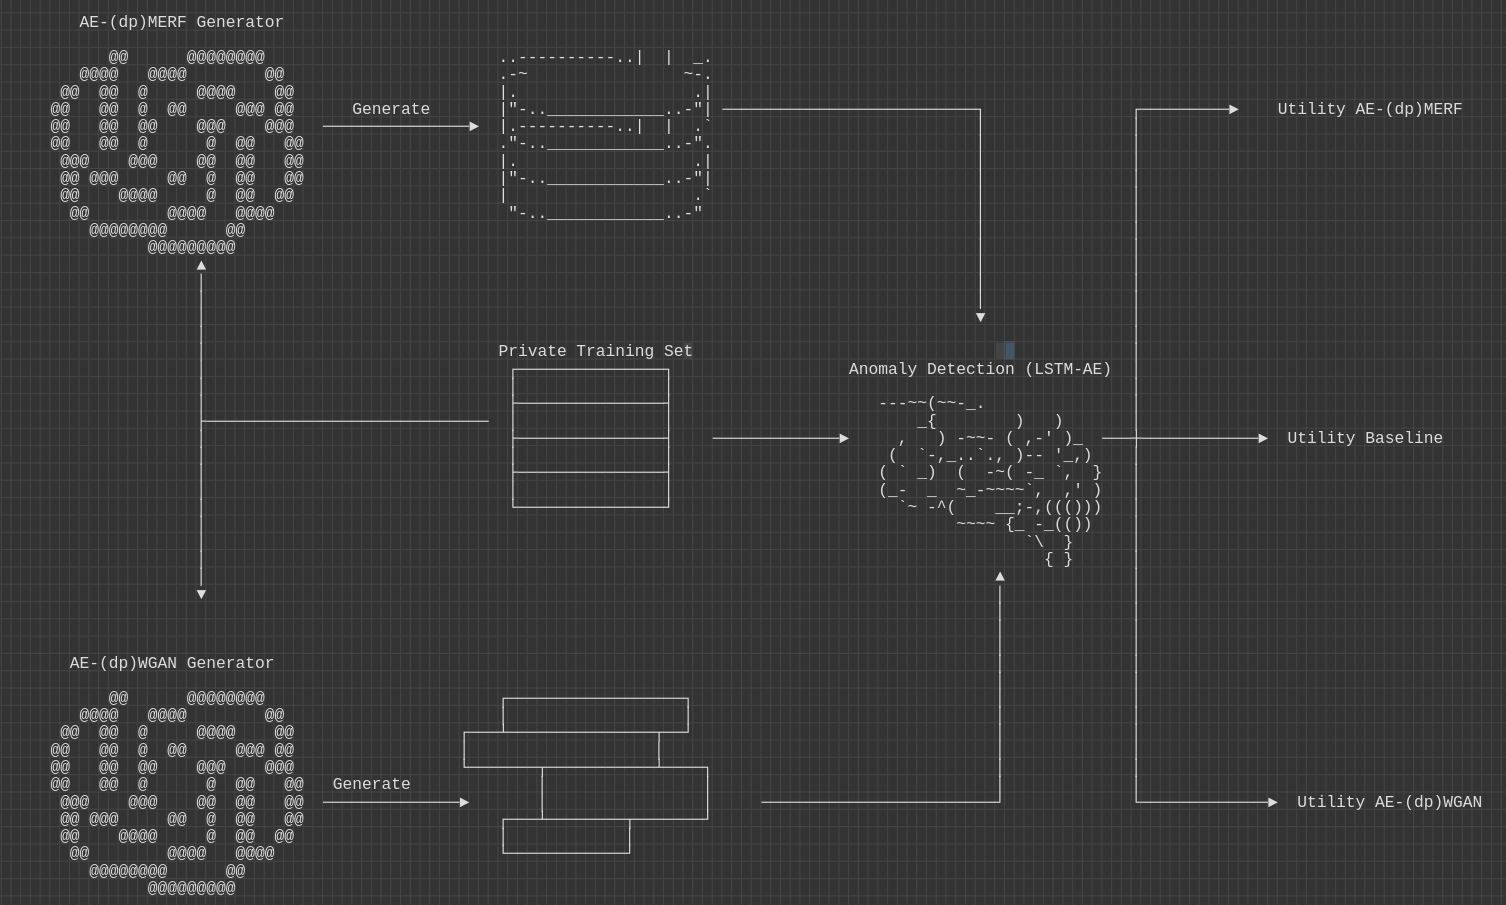
\includegraphics[scale=0.28]{str.png}
    \end{figure}
\end{frame}

\begin{frame}{Structure}
    \begin{enumerate}
        \item<1-> Train \alert{baseline model} for anomaly detection only on regular heartbeat data using an LSTM-AE.
        \item<2->  \alert{Generate heartbeat} data using two approaches:
        \begin{itemize}
            \item<2-> [--] AE-(dp)MERF
            \item<2-> [--] AE-(dp)WGAN
        \end{itemize}
        \item<3->  Train LSTM-AE for \alert{anomaly detection on synthetic data} and \alert{test on real}.
        \item<3-> Assess \alert{utility} by measuring performance for anomaly detection (Accuracy, precision, recall, F1). 
        \item<4->  \alert{Contaminate} training data with anomalous heartbeats and repeat.
    \end{enumerate}
\end{frame}




	\section[Lax-Wendroff-Verfahren ]{Lax-Wendroff-Verfahren}
	\section{Dataset: MITBIH ECG data}
\begin{frame}{Heartbeat Arrhythmia}
    \begin{figure}
        \centering
        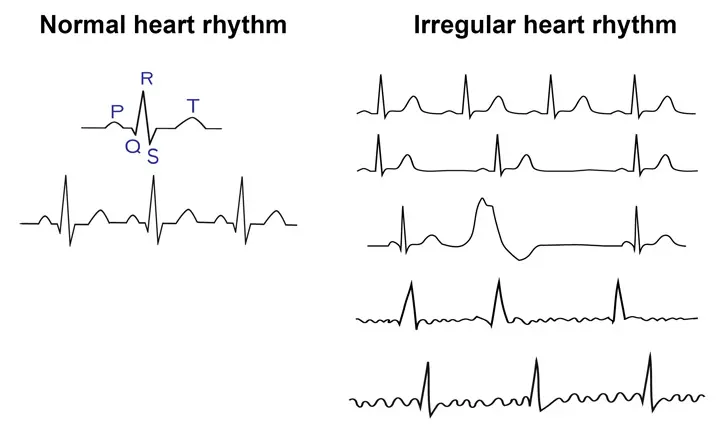
\includegraphics[scale=0.3]{images/heartbeat_arr.png}
        \caption[]{Different heartbeat arrhythmias \footnote{source: https://www.parkwayshenton.com.sg/health-plus/article/arrhythmia-guide}}
        \label{fig:enter-label}
    \end{figure}
\end{frame}

\begin{frame}{Arrhythmia Detection as an Anomaly Detection Problem}
We treat the problem of detecting irregular heartbeats as an anomaly detection problem from machine learning based on the reconstruction error:
\begin{itemize}
    \item<2->  We train a model \alert{on regular heartbeats} that is able to reconstruct that regular heartbeat.
    \item<3->  Given an irregular heartbeat the model should give \alert{higher reconstruction error}.
    \item<4->  Based on an optimal \alert{threshold} for that error we classify this heartbeat as either regular or irregular.
\end{itemize}
    \onslide<5>{Two reasons for this semi-supervised approach: high class imbalancy and no need for labelling.}
\end{frame} 

\begin{frame}{Baseline Model}
    Model is a LSTM-AE that is trained only on normal samples with the goal to reconstruct normal samples. The classification is made based on the reconstruction error.
    \begin{columns}
        \begin{column}{0.48\textwidth}
        \begin{figure}
            \centering
            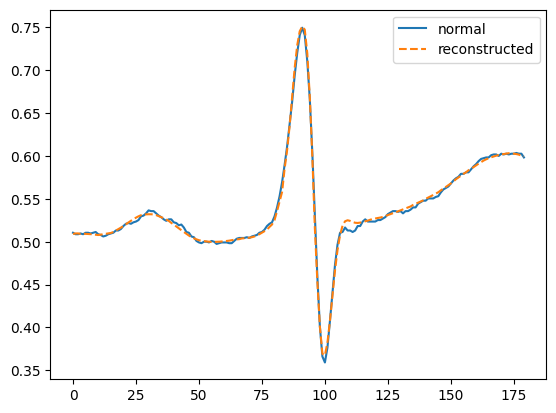
\includegraphics[scale=0.3]{images/rec_normal.png}
            \caption{reconstruction on normal sample \phantom{asdfsadf}}
            \label{fig:enter-label}
        \end{figure}
    \end{column}
    \begin{column}{0.48\textwidth}
        \begin{figure}
            \centering
            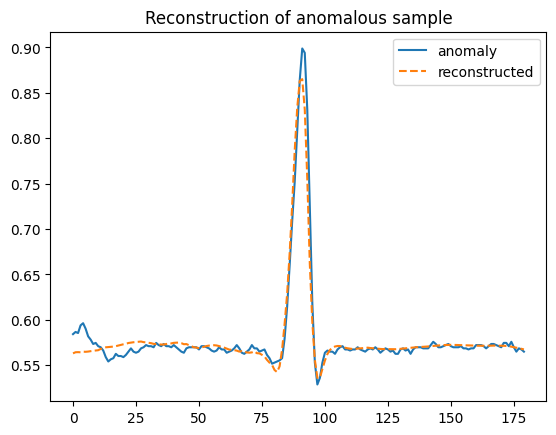
\includegraphics[scale=0.3]{images/rec_anom.png}
            \caption{reconstruction on anomalous sample}
            \label{fig:enter-label}
        \end{figure}
    \end{column}
    \end{columns}
\end{frame}

\begin{frame}
    \frametitle{Classification based on Reconstruction Error}

    \begin{columns}
        \begin{column}{0.48\textwidth}
        \begin{figure}
            \centering
            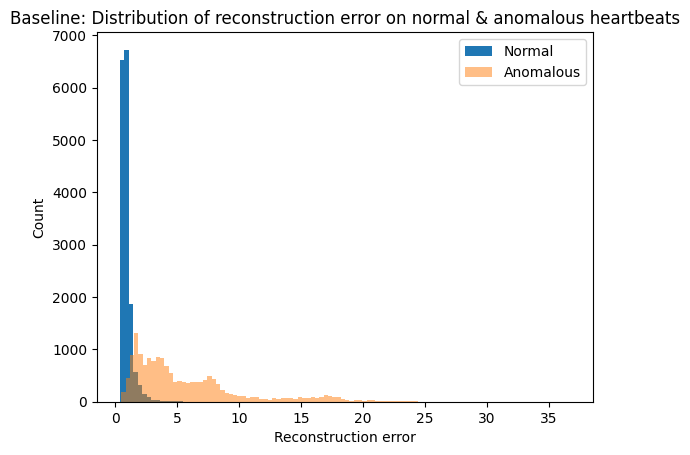
\includegraphics[scale=0.3]{hist_threshold_baseline.png}
            \caption{Distribution of reconstruction error on regular \& anomalous samples}
        \end{figure}
    \end{column}
    \begin{column}{0.48\textwidth}
        We can clearly see a \alert{difference in error distribution} for regular and anomalous samples. We choose the \alert{threshold that maximises the classification} accuracy.
    \end{column}
    \end{columns}

\end{frame}

	\clearpage

	\fancyhead[L]{ANHANG}
	\section*{Anhang}
	\addcontentsline{toc}{section}{Anhang}
	\section*{Appendix}

	\clearpage

	\pagestyle{fancy}
	\fancyhead[L]{LITERATURVERZEICHNIS}
	\fancyfoot[R]{\thepage}
	\printbibliography[heading=bibintoc, title=Literaturverzeichnis]
\end{document}
